% Chapter Template

\chapter{Introduction} % Main chapter title

\label{ch:introduction} % Change X to a consecutive number; for referencing this chapter elsewhere, use \ref{ChapterX}

%Surface normal is an important property of a surface with many applications, like surface reconstruction, shadings generation and other visual effects. However, the calculation of surface normal in many tasks is not as straightforward as simply the cross-product of two plane vectors. Especially in the task of real-world object digitalization, the surface is usually hardly to be mathematically described in equations due to the elaborate details on the objects. 
%
%Instead, it is common to infer it from the object point cloud. The point cloud records a great number of point positions on the object surface. These numbers of points altogether, are called point cloud, which is a memory economical solution to describe the shape of the object surface. They contains the geometry information of the surface, thus can be used for surface normal inference.
%




%
%Apart from this, due to the application scenarios, the working principle of scanners are various, which consequently produce point cloud structures in different forms. For the scanners without positions recording, the point cloud is unstructured. In this case, every 3D point can be captured by different capture position, and neighbors are not defined by capture time. It increases the difficulty and computation for the neighbor based normal inference approaches.  Furthermore, since the lack of inherent structure, the normal can hardly be inferred by the parallel approaches. 
%
%Thus getting a structured point cloud from a calibrated scanner is a much more convenient choice. One solution is the depth camera. It captures the RGB-D images of the object, which includes the standard RGB image with depth information of each pixel. Based on the calibrated camera, it is easy to acquire the structured surface point cloud from depth map and camera matrix. Furthermore, the point cloud is mapped directly based on the 2D depth map with the same capture position. which keeps the neighbor information of each point.  It is identical to the corresponding pixel in the 2D depth map. This provides a better view for the normal inference task since the neighbor information can be considered as a reference. 
%
%Besides geometry based approach, photometric stereo based approach using a set of light sources with knowing positions to separately project lights on the object, the surface normal can be calculated from the captured images and the known light directions. It is different from geometry based approach since no surface position is required. However, it usually require many different light positions to acquire a good performance \cite{spline-net} \cite{CNN-PS}, which raise the complexity for the data collection.
%
%Actually, the depth camera is able to acquire both geometry information like depth map as well as the images as photometric information. They are usually acquired at the same time when we collect the data. This inspired us to utilize the both depth map and image information to infer the surface map in order to find a more practical and more accurate approach that integrate two kinds of information and consequently improved surface normal inference.
%
%
%Deep learning based methods provides multiple possible solutions for the challenges mentioned above. First, to deal with the noised input, deep learning based methods already have the solution for the similar tasks like image inpainting and depth density enhancement, which base on the noised image as input to predict the clean and fully dense output with or without original meanings. Therefore, it can be a help for noise in the depth map. Besides, the network of deep learning model can also handle the structured point cloud as a single input and infer the corresponding normal all together, which is very time economical comparing to the approaches like neighbor based methods. In addition, the multi-stages training architectures provide a way to consider both depth map and texture image as the input to predict the surface normals, which not only consider the point cloud but also the add the lambertian reflection as a further constraint.
%
%Unfortunately, in the actual situation, the depth maps captured by the sensors are only semi-dense, which is mainly caused by. Consequently, it disrupts the robustness of the normal inference methods. Median filters can be used for the sparse missing pixels, however, for the case of huge missing holes in the depth map, it produces just a paltry result. Thus a reasonable guess is required for missing areas.
%
%
%In this work, we focus on the normal inference based on a semi-dense depth map with RGB image using deep learning based approaches. Specifically, the missing pixels in the depth map is filled up by the gated convolution and propagate in a customized UNet with skipping connections. The output of the training model is directly the surface normal corresponding the input depth map. The grayscale image is used to further improve the estimation accuracy. 
%For the training work, a dataset named “synthetic50-5” is created including 55 high resolution point clouds from internet, as shown in Appendix A. The point clouds provide with the high accurate normals, which can be used as the ground truth of the training work. Most of the models have elaborate details with high curvatures but also contain smooth surfaces. The trained model is evaluated on both synthetic dataset as well as the real dataset captured from RGB-D cameras. A series of metrics have been used for qualitative evaluation. The model is shown to achieve a remarkably better prediction accuracy at a low computational cost compared to the standard approaches for semi-dense point clouds.  

%% main problem, introduce deep learning, UNet

In 3D computer vision tasks, the \textit{point cloud} (i.e., an unstructured set of 3D points representing the surfaces in the scene) is a common input file to describe the object surface. Based on the geometry information in the point cloud, we can calculate the corresponding surface normal, which is an important feature in computer vision. The surface normal can be used for surface reconstruction, shading generation and other visual effects. The common method for determining the surface normal from the point cloud is the optimization approach, which considers the neighboring points in the same plane and calculates the surface normal. 

However, for single input data with only one shot, such as the data acquired by a depth camera, the point cloud is converted from a depth map and the given calibration information. In the case of active depth sensors, the depth map is usually only semi-dense due to optical noise and reflections in dark and shiny areas of the object surface, missing many pixels and holes. This limits the neighborhood-based approach because the missing data results in a smaller number of neighbors for each point. However, recent advances in the field of image inpainting have motivated researchers to use deep neural networks to recover the missing regions in the input data and achieve good performance. For example, \cite{gconv} uses a gated convolution network to recover user-defined removed regions in the images. \cite{nconv} uses a normalized convolution network to extend the semi-dense depth map to a fully dense depth map. In both cases, incomplete input data is used and converted to a fully dense output. Therefore, a Deep Learning based approach can be a way to deal with semi-dense depth maps for surface normal estimation tasks.

\begin{figure}[h!]
	\centering
	\captionsetup{width=\linewidth}
	{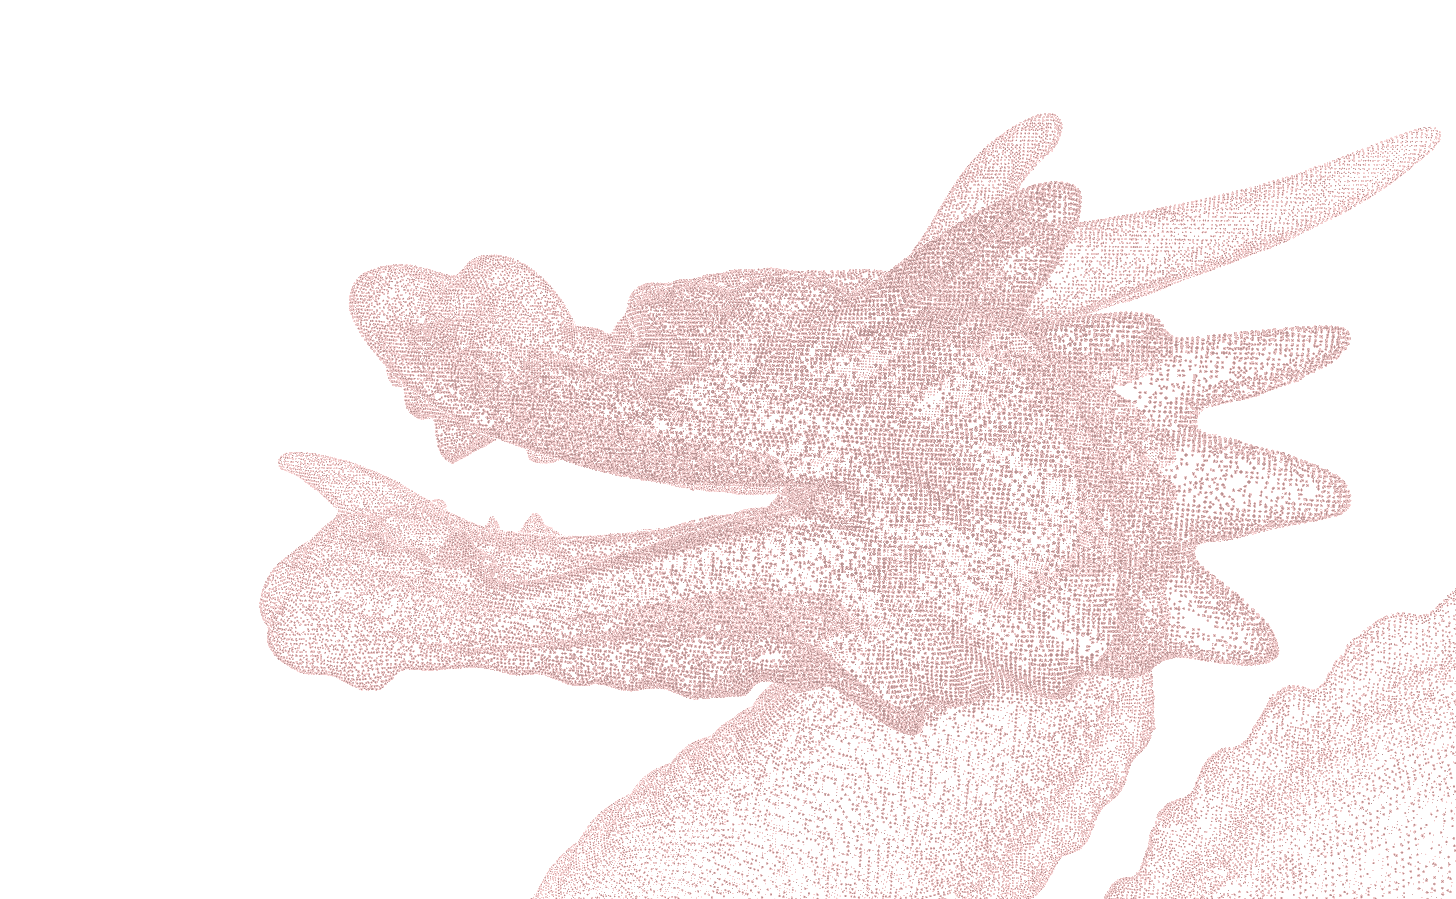
\includegraphics[width=.49\textwidth]{./Figures/point-cloud.png}}
	{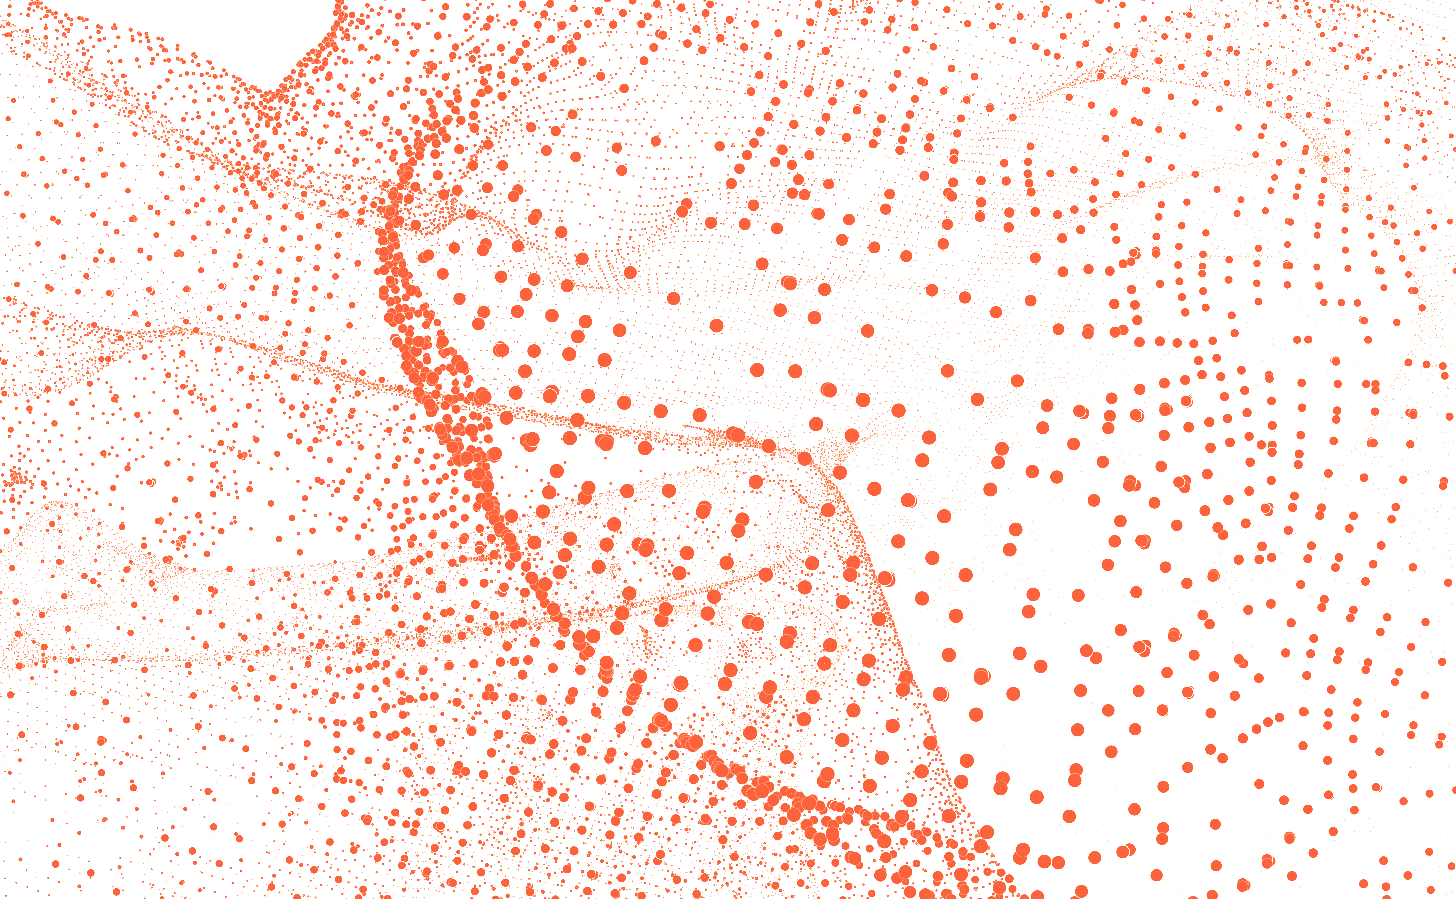
\includegraphics[width=.49\textwidth]{./Figures/point-cloud-zoom-in.png}}
	\decoRule
	\caption{Left: A portion of the point cloud of the \textit{dragon} object. Right: Zoom in of the point cloud.}
	\label{fig:point-cloud}
\end{figure}

%% introduce photometric stereo
Photometric stereo is another approach in computer vision that can be used for estimating surface normals, where the normals are derived from appearance variations under different illuminations. The corresponding methods are usually solved using the least squares problem, which is based on the point-wise image formation model \cite{SFS} and on the assumption of the Lambert surface. However, the Lambert surface generally cannot account for global illumination effects, which is an unavoidable problem due to light interactions.

%% papers contribution, main work
Both of the above directions have been widely explored using deep learning approaches. However, the approach that considers both geometry and illuminated information for normal estimation remains insufficient. We present a Deep Learning based approach that considers both geometric and photometric information for normal inference. For practical reasons, we consider a semi-dense depth map with only one additional illuminated image based on the calibrated camera as input data to find a compromise between the two methods. 

%% introduce the network, trip-net, dataset
One of our challenges is to apply the semi-dense input data to the neural network in an image-aware manner. \textit{U-Net} is a good network for computer vision tasks with up-sampling requirements. We modified it with a gated activation unit called \textit{gated convolution layer (gconv)} to handle semi-dense input data. Another challenge is to merge the different feature maps of the input data to cooperatively improve the surface normal inference task. We propose a \textit{multi-fusion} scheme for integrating separate feature maps. We will show that this \textit{multi-fusion} design can be leveraged by combining different input data types and improving the performance of surface normal inference. To train our network, we create a synthetic RGB-D image dataset by using a light source and ambient light illumination to simulate application scenarios. To simulate depth maps in the real world, we added uniformly distributed drop-out noise to the input data, with the noise density controlled by a parameter.

%% experiments
We trained our models on our proposed synthetic dataset \textit{synthetic-50-5} and evaluated them on 6 different metrics. The results show that our approach based on calibrated illuminated RGB-D images further improves the normal accuracy. We also applied our model to a real dataset and compared it with the optimization-based approach.


The structure of the paper is as follows: In Chapter 2, we briefly discuss related work on the normal inference task. Chapter 3 briefly introduces a traditional optimization-based approach and photometric stereo, and then proposes two learning-based approaches for surface normal estimation. Chapter 4 presents the dataset created for the training work and its preprocessing. Chapter 5 analyzes the experiments and provides both qualitative and quantitative evaluations of the models. Chapter 6 is the summary of the entire thesis.
